%\op{Is it only validation? It seems that some of the paramters are also chosen based on these simulations. Also, the discussion seems to be using some parameters which are only made explicit later. For instance, in 7.1.2, the circuits with less than 1000 cells are described as useless for premium. The reson for that seems to only become clear when reading 8.3.1, which indicates that payments are made after 1000 cells. I wonder if, at the end of this section, and before the experimental analysis, it would make sense to add a frame that sums-up what protocol will be analyzed, including the parameters: what channels and circuits are created when, when is payment happening, when are channels closed, \dots}

\subsection{Data Collection}
\label{subsec:datacollection}

We deployed during two weeks a data collection system to look for empirical
temporal information about lifetime and bandwidth consumption in Tor circuits.
Our objective was to have a deeper understanding of typical Tor usage and
whether such usage can benefit from our channel-based payment system. For
example, these measurements might capture some notion about the type and
magnitude of potential premium traffic. We classify the traffic type based on
the service connection port. Besides the classical ports 80 and 443 used for web
traffic, we aggregate data from some other families including the WHOIS
protocol~\cite{daigle2004whois} and RWHOIS~\cite{williamson1994referral} from
ports 43 and 4321, respectively. The complete list of families is constructed
from the reduced exit policies which we run on our relays. This measurement
methodology allows us to reason based on application specific traffic.

% We interested to know about the distribution lifetime of Tor circuits for each
% port we allow. We are also interested to picture how many cells those circuits
% handled through their lifetime with some level of granularity.

\paragraph*{Efforts to preserve users privacy}

To ensure ethical experimentation, we first contacted the Tor research safety
board~\cite{torsafety}. The feedback we received was subsequently used to
refactor our data collection process (e.g., no metadata from any specific flow
or circuit should be written on disk).

Data from five old and very stable exit relays with a total bandwidth of 50
MiB/s was collected, stripped of origin metadata, and aggregated on a central
server. The data collected from each relay is itself aggregated in memory. We
only collect data for circuits which are ``active'' from the perspective of the
exit relay, in other words, circuits which have received a connection request to
an IP address on the internet.
%The data collection is probabilistic; only 30\% of the circuits processed by our
%relays were considered in order to maintain plausible deniability on the
%clients' behalf.
Data is aggregated into bins of configurable size for every different traffic
family we consider. Once we collected enough data (1600 circuits) from a single
family, we dump the information on the disk, clear the relay memory, and resume
a new session. The final result is aggregated data containing the follow two
pieces of information for each pool:

\begin{itemize}
\item \textbf{Time Profile}: The number summing inbound and outbound cells in each
  5-second time interval since the success of the DNS request.

\item \textbf{Total Counts}: The total amount of cells processed by a circuit.
  We aggregate this information by taking the mean of fixed-size nearest
  neighbor bins.
\end{itemize}

Crucially, we do not record information linked to any single particular user
flow on disk.
%The code used for the data collection will be made available for
%audit online.

\paragraph*{Observations}

\begin{figure*}[t] \centering
\begin{subfigure}[t]{0.47\textwidth} \centering\centering
  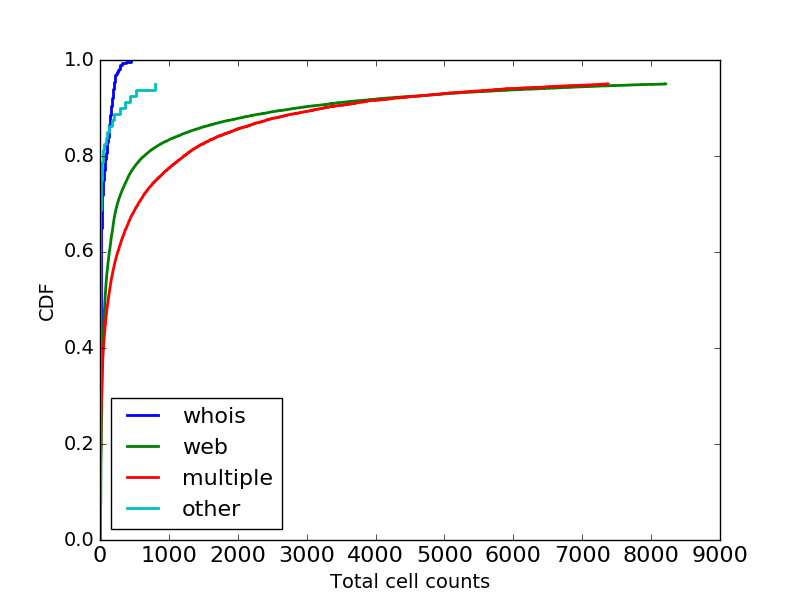
\includegraphics[width=0.7\textwidth]{images/totcellcountscdf.png}
  \caption{Total Counts --- Distribution of circuit size with respect to the
    total number of cells processed}
\label{fig:statsb}
\end{subfigure}
\begin{subfigure}[t]{0.47\textwidth} \centering
  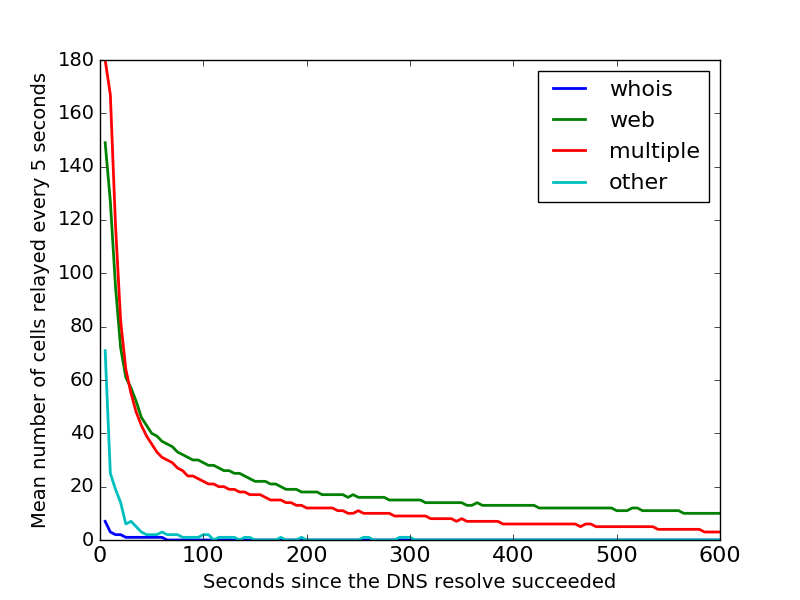
\includegraphics[width=0.7\textwidth]{images/exitmeasurement.png}
  \caption{Time Profile --- Average distribution of traffic across circuit
    lifetime beginning with the first DNS request.}
  \label{fig:statsa}
\end{subfigure}
\caption{Data collection from 5 old and stable exit relays with a cumulative
  bandwidth of $\approx$50 MiB/s}
\label{fig:stats}
\end{figure*}


Our measurements successfully captured several important pieces of information
for the design and justification of moneTor. For example, one important task is
to determine the number of potential users that could benefit from paid traffic.
From Figure~\ref{fig:statsb}, we observe that $\approx 82\%$ of circuits
carrying only web traffic exchanged less than 1000 cells. While we cannot deduce
any statements about users, we can speak to the fraction of circuits that may
benefit from a payment channel in the Tor network, since around $50\%$ of them
do not carry data and less than $17\%$ of them carry at least one web page. The
remaining $18\%$ would appear to be better candidates for moneTor.

It is also evident from Figure~\ref{fig:statsa} that most of the traffic is
usually carried within the first few tens of seconds regardless of traffic type.
From that result, we believe that the reliability of payment is critical within
the first few seconds, especially from a relay viewpoint. This result highlights
our choice to extend Bolt to offer high fairness. Furthermore, the front-loaded
distribution curve indicates a need to establish available payment channels as
soon as the user opens a circuit. As a result, we base our design upon a
preemptive circuit build strategy which serves to effectively eliminate channel
setup/establish latency in the average case.

%% In another area of research, it may be interesting to point out that since %
%$\approx 50\%$ of users do not carry data after their DNS request, some %
%adversary doing end-to-end correlation may prefer to use active attacks over %
%passive correlation to capture more identities.

